\chapter*{Dodatak: Prikaz aktivnosti grupe}
		\addcontentsline{toc}{chapter}{Dodatak: Prikaz aktivnosti grupe}
		
		\section*{Dnevnik sastajanja}
  
		\begin{packed_enum}
			\item  sastanak
			
			\item[] \begin{packed_item}
				\item Datum: 20. listopada 2022.
				\item Prisustvovali: svi članovi tima
				\item Teme sastanka:
				\begin{packed_item}
					\item  sastanak s asistentom i demonstratorom
					\item  analiziranje zadatka
                        \item razrješavanje nejasnoća i osnovnih dilema funkcionalnosti
				\end{packed_item}
			\end{packed_item}
			
			\item  sastanak
			\item[] \begin{packed_item}
				\item Datum: u ovom formatu: 21. listopada 2022.
				\item Prisustvovali: svi članovi tima
				\item Teme sastanka:
				\begin{packed_item}
					\item  podjela dužnosti i zadataka za naredni tjedan
					\item  konačan izbor alata i tehnologija
				\end{packed_item}
			\end{packed_item}

                \item  sastanak
			\item[] \begin{packed_item}
				\item Datum: 01. studenoga 2022.
				\item Prisustvovali: svi članovi tima
				\item Teme sastanka:
				\begin{packed_item}
					\item  izrada baze podataka
					\item  daljnja podjela rada (raspisivanje dokumentacije i izrada sekvencijskih i dijagrama obrazaca uporabe)
				\end{packed_item}
			\end{packed_item}

                \item  sastanak
			\item[] \begin{packed_item}
				\item Datum: 03. studenoga 2022.
				\item Prisustvovali: svi članovi tima
				\item Teme sastanka:
				\begin{packed_item}
					\item  drugi sastanak s asistentom i demonstratorom
					\item  komentiranje napisane dokumentacije i dijagrama
                        \item  daljnja podjela rada (front end i back end)
				\end{packed_item}
			\end{packed_item}

                \item  sastanak
			\item[] \begin{packed_item}
				\item Datum: 14. studenoga 2022.
				\item Prisustvovali: Bojan Puvača, Jurica Uglešić, Antonio Mišić, Matija Jelavić
				\item Teme sastanka:
				\begin{packed_item}
					\item  izrada dijagrama razreda
                        
				\end{packed_item}
			\end{packed_item}
   
                \item  sastanak
			\item[] \begin{packed_item}
				\item Datum: 11. prosinca 2022.
				\item Prisustvovali: svi članovi tima
				\item Teme sastanka:
				\begin{packed_item}
					\item  podjela rada (podjela posla na frontend i backend po ekranima
                        
				\end{packed_item}
			\end{packed_item}
   
                \item  sastanak
			\item[] \begin{packed_item}
				\item Datum: 17. prosinca 2022.
				\item Prisustvovali: svi članovi tima
				\item Teme sastanka:
				\begin{packed_item} 
                        \item  prezentacija napravljenog ostalim članovima tima
                        \item daljnja podjela zadataka
                        
				\end{packed_item}
			\end{packed_item}

                \item  sastanak
			\item[] \begin{packed_item}
				\item Datum: 21. prosinca 2022.
				\item Prisustvovali: Antonio Mišić, Ema Vlainić, Jurica Uglešić
				\item Teme sastanka:
				\begin{packed_item} 
                        \item  prezentacija alfa inačice projekta asistentu i demonstratoru
				\end{packed_item}
			\end{packed_item}
   
                \item  sastanak
			\item[] \begin{packed_item}
				\item Datum: 05. siječnja 2023.
				\item Prisustvovali: svi članovi tima
				\item Teme sastanka:
				\begin{packed_item} 
                        \item  dorađivanje alfa inačice
                        \item  podjela pisanja dokumentacije
                        \item  komentiranje izrade dijagrama stanja, komponenti i aktivnosti
				\end{packed_item}
			\end{packed_item}

                \item  sastanak
			\item[] \begin{packed_item}
				\item Datum: 02. siječnja 2023.
				\item Prisustvovali: svi članovi tima
				\item Teme sastanka:
				\begin{packed_item} 
                        \item  dorađivanje alfa inačice
                        \item  podjela pisanja dokumentacije
                        \item  komentiranje izrade dijagrama stanja, komponenti i aktivnosti
				\end{packed_item}
			\end{packed_item}

                \item  sastanak
			\item[] \begin{packed_item}
				\item Datum: 05. siječnja 2023.
				\item Prisustvovali: Bojan Puvača, Matija Jelavić
				\item Teme sastanka:
				\begin{packed_item} 
                        \item  sastanak s asistentom i demonstratorom
                        \item  komentiranje izrade dijagrama i implementacije projekta
				\end{packed_item}
			\end{packed_item}

                \item  sastanak
			\item[] \begin{packed_item}
				\item Datum: 09. siječnja 2023.
				\item Prisustvovali: Bojan Puvača, Antonio Mišić, Matija Jelavić
				\item Teme sastanka:
				\begin{packed_item} 
                        \item  ispravljanje funkcija na backendu
				\end{packed_item}
			\end{packed_item}

                \item  sastanak
			\item[] \begin{packed_item}
				\item Datum: 12. siječnja 2023.
				\item Prisustvovali: svi članovi tima
				\item Teme sastanka:
				\begin{packed_item} 
                        \item  zadnji sastanak s asistentom i demonstratorom
                        \item  prezentacija projekta
				\end{packed_item}
			\end{packed_item}
			
			%
			
		\end{packed_enum}
		
		\eject
		\section*{Tablica aktivnosti}

			\begin{longtblr}[
					label=none,
				]{
					vlines,hlines,
					width = \textwidth,
					colspec={X[7, l]X[1, c]X[1, c]X[1, c]X[1, c]X[1, c]X[1, c]X[1, c]}, 
					vline{1} = {1}{text=\clap{}},
					hline{1} = {1}{text=\clap{}},
					rowhead = 1,
				} 
				\multicolumn{1}{c|}{} & \multicolumn{1}{c|}{\rotatebox{90}{\textbf{Bojan Puvača}}} & \multicolumn{1}{c|}{\rotatebox{90}{\textbf{Matija Jelavić}}} &	\multicolumn{1}{c|}{\rotatebox{90}{\textbf{Danijel Kovačević}}} & \multicolumn{1}{c|}{\rotatebox{90}{\textbf{Antonio Mišić}}} &	\multicolumn{1}{c|}{\rotatebox{90}{\textbf{Katarina Šabić}}} & \multicolumn{1}{c|}{\rotatebox{90}{\textbf{Jurica Uglešić}}} &	\multicolumn{1}{c|}{\rotatebox{90}{\textbf{Ema Vlainić}}} \\  
				Upravljanje projektom 		& 8 &  &  &  &  &  & \\ 
				Opis projektnog zadatka 	&  &  &  &  &  & 2 & \\ 
				
				Funkcionalni zahtjevi       & 2 &  &  &  & 1 &  &  \\ 
				Opis pojedinih obrazaca 	&  &  & 4 &  & 3 &  &  \\ 
				Dijagram obrazaca 			&  & 6 &  &  &  &  &  \\ 
				Sekvencijski dijagrami 		&  &  &  &  &  &  & 6 \\ 
				Opis ostalih zahtjeva 		&  &  &  &  &  & 1 &  \\ 

				Arhitektura i dizajn sustava	 &  &  &  & 2 &  &  &  \\ 
				Baza podataka				&  &  & 2 &  &  &  &   \\ 
				Dijagram razreda 			&  & 2 & 2 & 2 &  & 2 &   \\ 
				Dijagram stanja				&  &  &  &  & 5 &  &  \\ 
				Dijagram aktivnosti 		&  &  &  &  &  & 3 &  \\ 
				Dijagram komponenti			&  &  & 3 &  &  &  &  \\ 
				Korištene tehnologije i alati 		&  &  & 1 &  &  &  &  \\ 
				Ispitivanje programskog rješenja 	&  &  & 2 & 8 &  &  &  \\ 
				Dijagram razmještaja			&  &  &  &  &  & 1 &  \\ 
				Upute za puštanje u pogon 		&  &  &  &  &  &  &  \\  
				Dnevnik sastajanja 			&  &  &  &  & 4 &  &  \\ 
				Zaključak i budući rad 		&  &  &  &  &  & 1 &  \\  
				Popis literature 			&  &  &  &  &  &  &  \\  
				&  &  &  &  &  &  &  \\ \hline 
				\textit{Dodatne stavke kako ste podijelili izradu aplikacije} 			&  &  &  &  &  &  &  \\ 
				Izrada početne stranice				&  &  &  &  &  &  & 6 \\  
				Izrada baze podataka 		 			& 1 & 1 & 1 & 1 & 1 & 1 & 1\\  
				Spajanje s bazom podataka 							& 6 &  &  &  &  &  &  \\ 
				Backend							& 3 & 12 &  & 15 &  & 6 &  \\ 
                Frontend							& 20 &  &  &  & 7 &  & 15 \\
                Registracija, validacija, prijava korisnika u sustav 							& 6 &  &  &  & 6 &  &  \\  
                Puštanje aplikacije u pogon							& 13 &  &  &  &  &  &  \\  

				 							&  &  &  &  &  &  &\\ 
			\end{longtblr}
					
	
		\eject
        
		\section*{Dijagrami pregleda promjena}


            \begin{figure}[H] 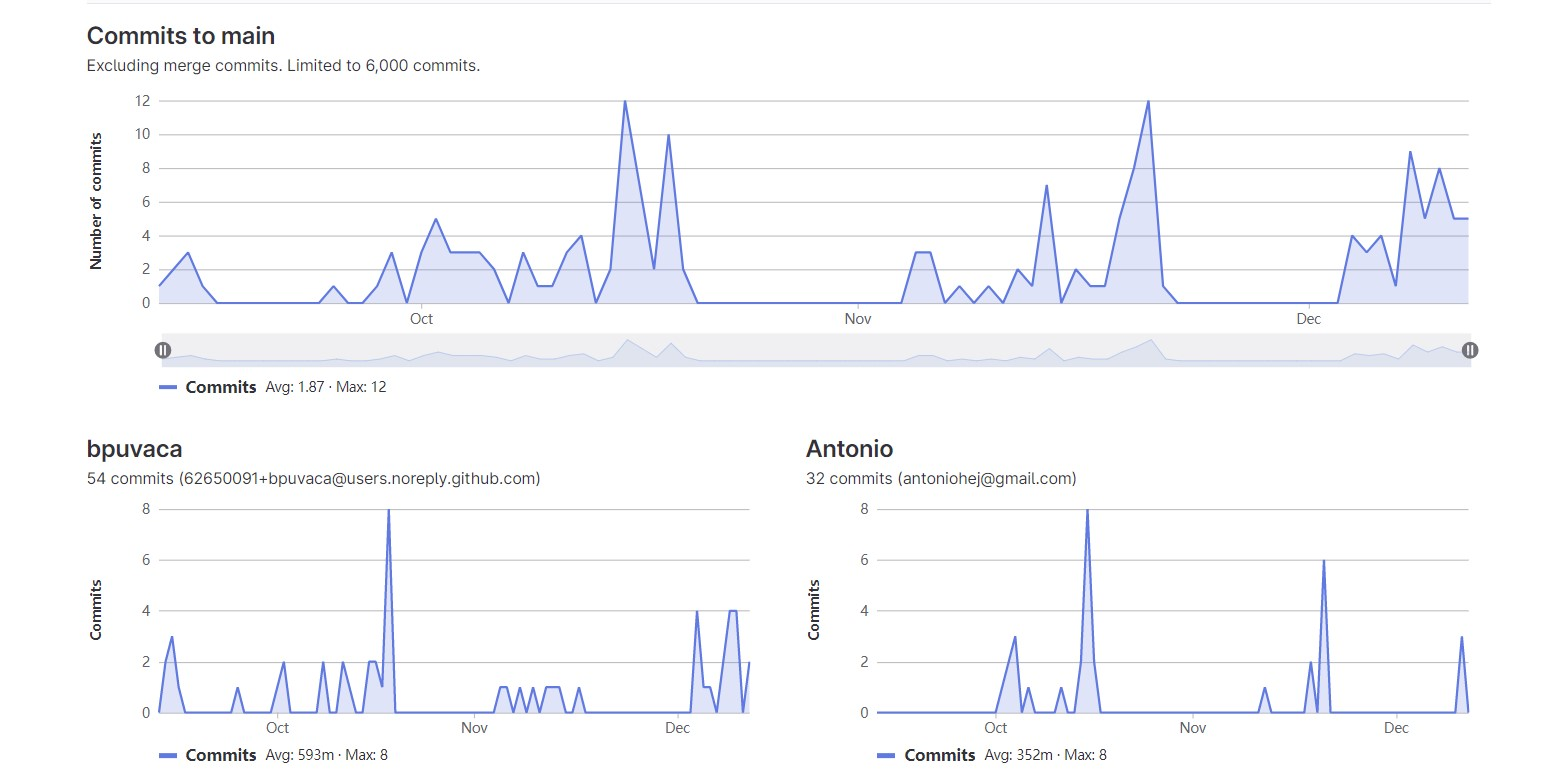
\includegraphics[width=\linewidth]{slike/pregledpromjena1.jpg}
				\caption{Prikaz aktivnosti na repozitoriju}
			\end{figure}

            \begin{figure}[H] 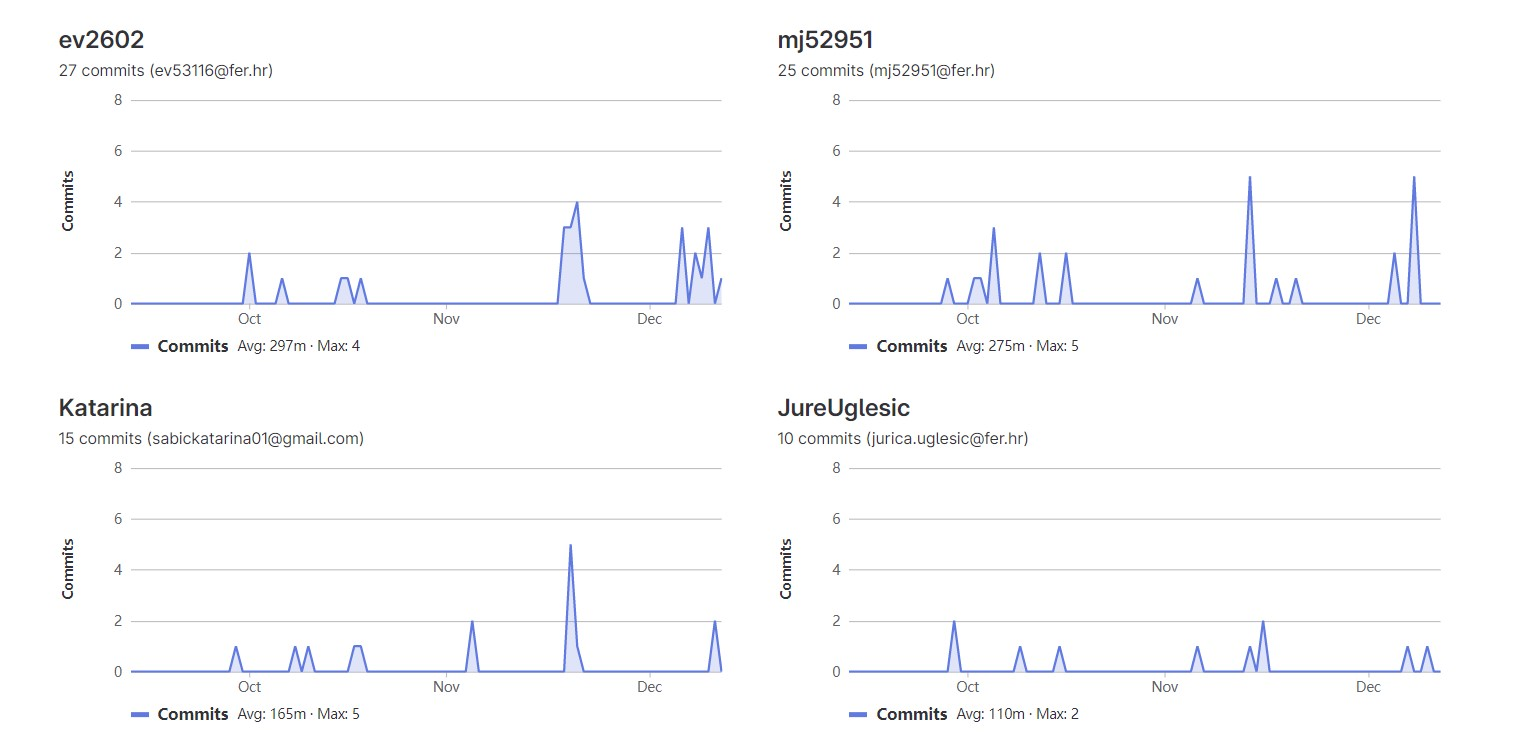
\includegraphics[width=\linewidth]{slike/pregledpromjena2.jpg}
				\caption{Prikaz aktivnosti na repozitoriju}
			\end{figure}

            \begin{figure}[H] 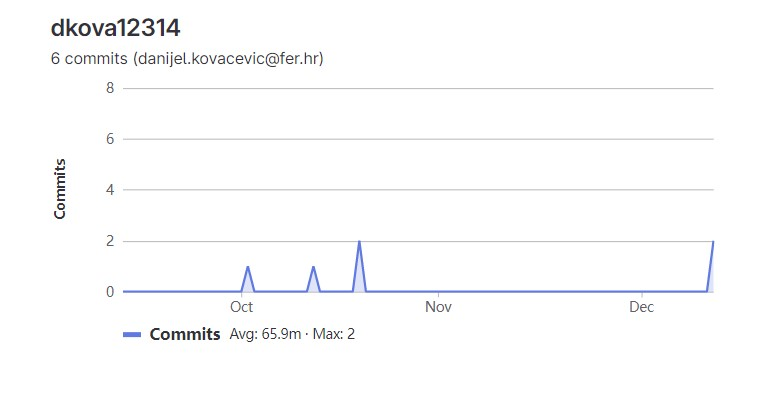
\includegraphics[width=\linewidth]{slike/pregledpromjena3.jpg}
				\caption{Prikaz aktivnosti na repozitoriju}
			\end{figure}
		
		
		
		
		
	    